\subsection{Basic facts of multiplication 乘法的基础}
\begin{paracol}{2}
Multiplication could be thought as a repeated addition. The multiplication of two numbers is equivalent to adding as many copies of one of them, the multiplicand, as the value of the other one, the multiplier. Consider the following
\switchcolumn[1]
乘法是可以用加法来表示的。两个数相乘相当于把被乘数加乘数次。例如
\end{paracol}
$$
8\times 4 = 32 \Leftrightarrow 8+8+8+8 = 32.
$$
\begin{paracol}{2}
Multiplicand and multiplier are called factors of the result. 
\switchcolumn[1]
乘数和被乘数都是乘积的因子。
\switchcolumn[0]*
For the mutiplication within 10, it is better to remember all of the results. 
\switchcolumn[1]
我们最好能都熟练的掌握10以内的数的乘法的结果。
\end{paracol}

\begin{figure}[!hbtp]
\centering
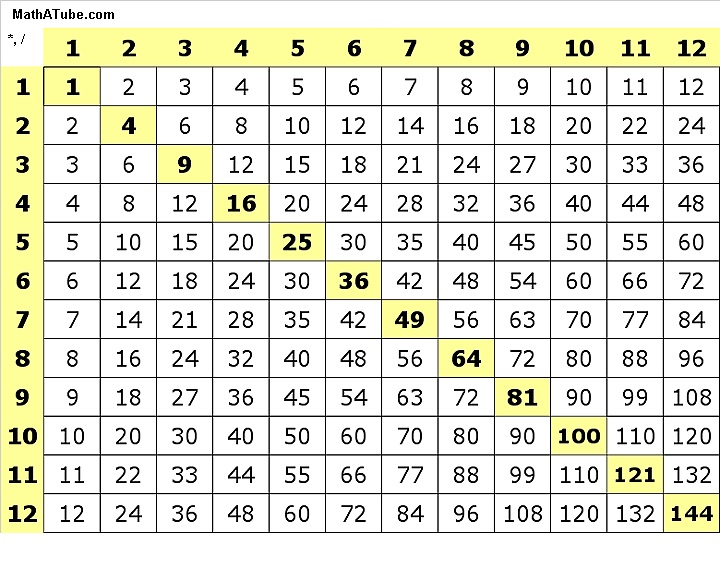
\includegraphics[width=0.7\textwidth]{timesanddivisiontablechart.jpg}
\caption{Multiplication chart\label{figur:multichart}}
\end{figure}


\begin{figure}[!hbtp]
\centering
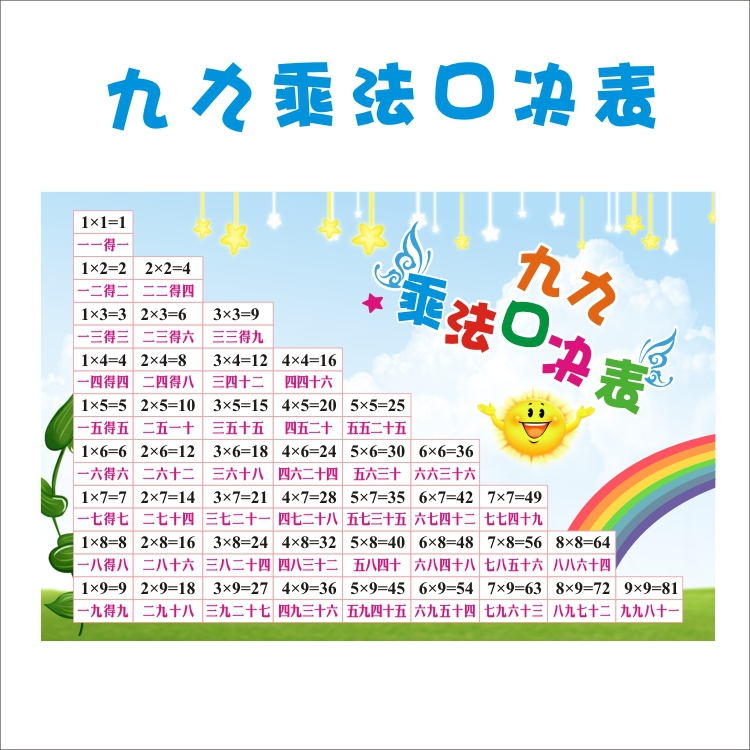
\includegraphics[width=0.6\textwidth]{99multi.jpg}
\caption{九九乘法口诀表\label{figur:multichart1}}
\end{figure}

\subsection{Long multiplication  乘法竖式}

\begin{paracol}{2}
Long multiplication is a method used to solve the multiplication problems with large numbers. One thing can really help you in long multiplication is if you know the multiplication chart by heart. This will speed up your work and make it more accurate. 
\switchcolumn[1]
乘法竖式是用来计算较大数的乘法。如果我们可以牢记上面的乘法表,可以帮助我们更快速准确的进行竖式运算。
\end{paracol}

\paragraph{Multi-digit number times 1-digit number 多位数乘一位数}
\ \ 

\begin{paracol}{2}
The key of the multiplication is that multiplying each place value of the multi-digit number by the one-digit number and suming up the results.
\switchcolumn[1]
如果是多位数乘一位数,就用多位数中的每一位分别乘那个一位数,然后把结果相加。
\switchcolumn[0]*
\begin{description}
\item [{\bf Step 1:} ] write down the numbers on top of each other. Make sure  align the numbers on the right.
\item [{\bf Step 2:} ] Multiply each place value of the multiplicand by the 1-digit multiplier. 
\item [{\bf Step 3:} ] Align the result with the corresponding place. For exampe, multiply ones by the 1-digit number, then align the result with ones. Add the carry on numbers from the previous.
\end{description}
\switchcolumn[1]
\begin{description}
\item [{\bf 第一步:} ] 写竖式,相同数位对齐;
\item [{\bf 第二步:} ] 多位数每一位上的数分别与这个一位数相乘,从多位数个位起;
\item [{\bf 第三步:} ] 乘到哪一位就把结果写在哪一位数相应的位置上。注意加上上次计算的进位。
\end{description}
\end{paracol}

\begin{example}
$284\times 3$
\end{example}
%\multicolumn{3}{c}{\fcolorbox{black}{black}{\color{white}\ \ \ Step 1\ \ \ }}\\
\begin{solution}
$$
\begin{array}{lccc}
&2&8&4\\
\times&&&3\\
\hline
&&&
\end{array}
\Rightarrow
\begin{array}{lccc}
&2&8&{\color{red} \bm 4}\\
\times&&_{\color{red}1}&{\color{red} \bm 3}\\
\hline
&&&{\color{red} \bm 2}
\end{array}
$$
$$
\Rightarrow
\begin{array}{lccc}
&2&{\color{red} \bm 8}&4\\
\times&_{\color{red} \bm 2}&_{1}&{\color{red} \bm 3}\\
\hline
&&{\color{red} \bm 5}&2\\
\end{array}
\Rightarrow
\begin{array}{lccc}
&{\color{red} \bm2}& 8&4\\
\times&_{2}&_{1}&{\color{red} \bm 3}\\
\hline
&{\color{red} \bm 8}& 6&4
\end{array}
$$
$284\times 3= 864.$
\end{solution}

\paragraph{Multi-digit number times multi-digit number 多位数乘多位数}
\ \  

\begin{paracol}{2}
The multiplication bewteen two multi-digit numbers is based on the multiplication between multi-digit number and 1-digit number. The rule is as follows.
\switchcolumn[1]
多位数多位数乘法法则是基于多位数一位数的乘法。其法则如下:
\switchcolumn[0]*
\begin{description}
\item [{\bf Step 1:} ] write down the numbers on top of each other. It is better to write down the number with more digits on the top.
\item [{\bf Step 2:} ] Multiply the multiplicand by ones of the multiplier and align the ones of the results to the ones under the line. Then multiply the multiplicand by tens of the multiplier and align the ones of the results to the tens under the line. And so on.
\item [{\bf Step 3:} ] Sum all of the results up.
\end{description}
\switchcolumn[1]
\begin{description}
\item [{\bf 第一步:} ] 写竖式,最好把数位较多的乘数写在上面作为被乘数,数位较少的写在下面;
\item [{\bf 第二步:} ] 用被乘数与乘数的个位相乘,把相乘得到的积的末位写在个位上;然后再与十位上的数相乘写在十位上,... ...
\item [{\bf 第三步:} ] 把每次乘得的数相加得到最终结果。
\end{description}
\end{paracol}

\begin{example}
$125\times 124$
\end{example}
\begin{solution}
$$
\begin{array}{lccc}
&1&2&5\\
\times&1&2&4\\
\hline
&&&
\end{array}
\Rightarrow
\begin{array}{lccc}
&{\color{red} \bm 1}&{\color{red} \bm 2}&{\color{red} \bm 5}\\
\times&1&2&{\color{red} \bm 4}\\
\hline
&{\color{red} \bm 5}&{\color{red} \bm 0}&{\color{red} \bm 0}
\end{array}
$$
$$
\Rightarrow
\begin{array}{ccccc}
&&{\color{red} \bm 1}&{\color{red} \bm 2}&{\color{red} \bm 5}\\
\times&&1&{\color{red} \bm 2}&4\\
\hline
&&5&0&0\\
&{\color{red} \bm 2}&{\color{red} \bm 5}&{\color{red} \bm 0}&\\
&&&&\\
&&&&
\end{array}
\Rightarrow
\begin{array}{ccccc}
&&{\color{red} \bm 1}&{\color{red} \bm 2}&{\color{red} \bm 5}\\
\times&&{\color{red} \bm 1}&2&4\\
\hline
&&5&0&0\\
&2&5&0&\\
{\color{red} \bm 1}&{\color{red} \bm 2}&{\color{red} \bm 5}&&\\
&&&&
\end{array}
\Rightarrow
\begin{array}{ccccc}
&&1&2&5\\
\times&&1&2&4\\
\hline
&&5&0&0\\
&2&5&0&\\
1&2&5&&\\
\hline
{\color{red} \bm 1}&{\color{red} \bm 5}&{\color{red} \bm 5}&{\color{red} \bm 0}&{\color{red} \bm 0}
\end{array}
$$
$125\times 124= 15,500.$
\end{solution}

\begin{paracol}{2}
There are some tricks to help do the multiplication faster and easier.

1. If there are zeros at the end of the number, we can leave them and multiply the remaining numbers. Then add the zeros. 
\switchcolumn[1]
要提高计算速度有以下一些技巧。

1. 末尾有0的数的乘法。可以先把0前面的数相乘再添0,得出结果。
\end{paracol}

\begin{example}
$2800\times 130$
\end{example}
\begin{solution}
$$
\begin{array}{cccc:cc}
&&2&8&0&\\
\times&&1&3&0&\\
\hline
&&8&4&&\\
&2&8&&&\\
\hline
&3&6&4&0&0\\
\end{array}
$$
$2800\times 130=36400$.
\end{solution}

\begin{paracol}{2}
2. If there are repeat numbers in the multiplier, you do not need to compute it again. 
\switchcolumn[1]
2. 当乘数有重复的数字时,不必重复相乘,可以直接写出后面的结果。只是要注意对齐。
\end{paracol}
\begin{example}
$315\times 66$
\end{example}
\begin{solution}
$$
\begin{array}{ccccc}
&&3&1&5\\
\times&&&6&6\\
\hline
&1&8&9&0\\
1&8&9&0&\\
\hline
2&0&7&9&0\\
\end{array}
$$
$315\times 66=20790$.
\end{solution}
   \newpage